% Created by tikzDevice version 0.12
% !TEX encoding = UTF-8 Unicode
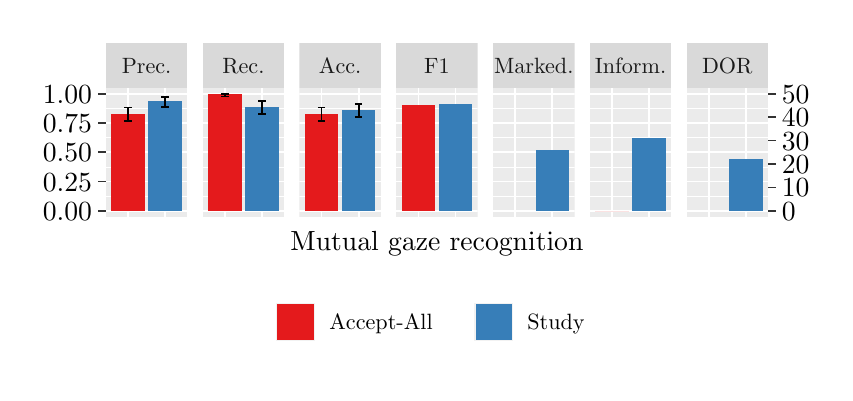
\begin{tikzpicture}[x=1pt,y=1pt]
\definecolor{fillColor}{RGB}{255,255,255}
\path[use as bounding box,fill=fillColor,fill opacity=0.00] (0,0) rectangle (288.00,124.59);
\begin{scope}
\path[clip] (  0.00,  0.00) rectangle (288.00,124.59);
\definecolor{drawColor}{RGB}{255,255,255}
\definecolor{fillColor}{RGB}{255,255,255}

\path[draw=drawColor,line width= 0.6pt,line join=round,line cap=round,fill=fillColor] (  0.00,  0.00) rectangle (288.00,124.59);
\end{scope}
\begin{scope}
\path[clip] ( 28.22, 56.29) rectangle ( 57.70,102.84);
\definecolor{fillColor}{gray}{0.92}

\path[fill=fillColor] ( 28.22, 56.29) rectangle ( 57.70,102.84);
\definecolor{drawColor}{RGB}{255,255,255}

\path[draw=drawColor,line width= 0.3pt,line join=round] ( 28.22, 63.69) --
	( 57.70, 63.69);

\path[draw=drawColor,line width= 0.3pt,line join=round] ( 28.22, 74.27) --
	( 57.70, 74.27);

\path[draw=drawColor,line width= 0.3pt,line join=round] ( 28.22, 84.85) --
	( 57.70, 84.85);

\path[draw=drawColor,line width= 0.3pt,line join=round] ( 28.22, 95.43) --
	( 57.70, 95.43);

\path[draw=drawColor,line width= 0.6pt,line join=round] ( 28.22, 58.40) --
	( 57.70, 58.40);

\path[draw=drawColor,line width= 0.6pt,line join=round] ( 28.22, 68.98) --
	( 57.70, 68.98);

\path[draw=drawColor,line width= 0.6pt,line join=round] ( 28.22, 79.56) --
	( 57.70, 79.56);

\path[draw=drawColor,line width= 0.6pt,line join=round] ( 28.22, 90.14) --
	( 57.70, 90.14);

\path[draw=drawColor,line width= 0.6pt,line join=round] ( 28.22,100.72) --
	( 57.70,100.72);

\path[draw=drawColor,line width= 0.6pt,line join=round] ( 36.26, 56.29) --
	( 36.26,102.84);

\path[draw=drawColor,line width= 0.6pt,line join=round] ( 49.66, 56.29) --
	( 49.66,102.84);
\definecolor{fillColor}{RGB}{228,26,28}

\path[fill=fillColor] ( 30.23, 58.40) rectangle ( 42.29, 93.51);
\definecolor{fillColor}{RGB}{55,126,184}

\path[fill=fillColor] ( 43.63, 58.40) rectangle ( 55.69, 98.27);
\definecolor{drawColor}{RGB}{0,0,0}

\path[draw=drawColor,line width= 0.6pt,line join=round] ( 48.32, 99.65) --
	( 51.00, 99.65);

\path[draw=drawColor,line width= 0.6pt,line join=round] ( 49.66, 99.65) --
	( 49.66, 96.02);

\path[draw=drawColor,line width= 0.6pt,line join=round] ( 48.32, 96.02) --
	( 51.00, 96.02);

\path[draw=drawColor,line width= 0.6pt,line join=round] ( 34.92, 95.72) --
	( 37.60, 95.72);

\path[draw=drawColor,line width= 0.6pt,line join=round] ( 36.26, 95.72) --
	( 36.26, 90.80);

\path[draw=drawColor,line width= 0.6pt,line join=round] ( 34.92, 90.80) --
	( 37.60, 90.80);
\end{scope}
\begin{scope}
\path[clip] ( 63.20, 56.29) rectangle ( 92.67,102.84);
\definecolor{fillColor}{gray}{0.92}

\path[fill=fillColor] ( 63.20, 56.29) rectangle ( 92.67,102.84);
\definecolor{drawColor}{RGB}{255,255,255}

\path[draw=drawColor,line width= 0.3pt,line join=round] ( 63.20, 63.69) --
	( 92.67, 63.69);

\path[draw=drawColor,line width= 0.3pt,line join=round] ( 63.20, 74.27) --
	( 92.67, 74.27);

\path[draw=drawColor,line width= 0.3pt,line join=round] ( 63.20, 84.85) --
	( 92.67, 84.85);

\path[draw=drawColor,line width= 0.3pt,line join=round] ( 63.20, 95.43) --
	( 92.67, 95.43);

\path[draw=drawColor,line width= 0.6pt,line join=round] ( 63.20, 58.40) --
	( 92.67, 58.40);

\path[draw=drawColor,line width= 0.6pt,line join=round] ( 63.20, 68.98) --
	( 92.67, 68.98);

\path[draw=drawColor,line width= 0.6pt,line join=round] ( 63.20, 79.56) --
	( 92.67, 79.56);

\path[draw=drawColor,line width= 0.6pt,line join=round] ( 63.20, 90.14) --
	( 92.67, 90.14);

\path[draw=drawColor,line width= 0.6pt,line join=round] ( 63.20,100.72) --
	( 92.67,100.72);

\path[draw=drawColor,line width= 0.6pt,line join=round] ( 71.24, 56.29) --
	( 71.24,102.84);

\path[draw=drawColor,line width= 0.6pt,line join=round] ( 84.64, 56.29) --
	( 84.64,102.84);
\definecolor{fillColor}{RGB}{228,26,28}

\path[fill=fillColor] ( 65.21, 58.40) rectangle ( 77.27,100.72);
\definecolor{fillColor}{RGB}{55,126,184}

\path[fill=fillColor] ( 78.61, 58.40) rectangle ( 90.66, 96.08);
\definecolor{drawColor}{RGB}{0,0,0}

\path[draw=drawColor,line width= 0.6pt,line join=round] ( 83.30, 98.01) --
	( 85.98, 98.01);

\path[draw=drawColor,line width= 0.6pt,line join=round] ( 84.64, 98.01) --
	( 84.64, 93.45);

\path[draw=drawColor,line width= 0.6pt,line join=round] ( 83.30, 93.45) --
	( 85.98, 93.45);

\path[draw=drawColor,line width= 0.6pt,line join=round] ( 69.90,100.72) --
	( 72.58,100.72);

\path[draw=drawColor,line width= 0.6pt,line join=round] ( 71.24,100.72) --
	( 71.24, 99.66);

\path[draw=drawColor,line width= 0.6pt,line join=round] ( 69.90, 99.66) --
	( 72.58, 99.66);
\end{scope}
\begin{scope}
\path[clip] ( 98.17, 56.29) rectangle (127.65,102.84);
\definecolor{fillColor}{gray}{0.92}

\path[fill=fillColor] ( 98.17, 56.29) rectangle (127.65,102.84);
\definecolor{drawColor}{RGB}{255,255,255}

\path[draw=drawColor,line width= 0.3pt,line join=round] ( 98.17, 63.69) --
	(127.65, 63.69);

\path[draw=drawColor,line width= 0.3pt,line join=round] ( 98.17, 74.27) --
	(127.65, 74.27);

\path[draw=drawColor,line width= 0.3pt,line join=round] ( 98.17, 84.85) --
	(127.65, 84.85);

\path[draw=drawColor,line width= 0.3pt,line join=round] ( 98.17, 95.43) --
	(127.65, 95.43);

\path[draw=drawColor,line width= 0.6pt,line join=round] ( 98.17, 58.40) --
	(127.65, 58.40);

\path[draw=drawColor,line width= 0.6pt,line join=round] ( 98.17, 68.98) --
	(127.65, 68.98);

\path[draw=drawColor,line width= 0.6pt,line join=round] ( 98.17, 79.56) --
	(127.65, 79.56);

\path[draw=drawColor,line width= 0.6pt,line join=round] ( 98.17, 90.14) --
	(127.65, 90.14);

\path[draw=drawColor,line width= 0.6pt,line join=round] ( 98.17,100.72) --
	(127.65,100.72);

\path[draw=drawColor,line width= 0.6pt,line join=round] (106.21, 56.29) --
	(106.21,102.84);

\path[draw=drawColor,line width= 0.6pt,line join=round] (119.61, 56.29) --
	(119.61,102.84);
\definecolor{fillColor}{RGB}{228,26,28}

\path[fill=fillColor] (100.18, 58.40) rectangle (112.24, 93.51);
\definecolor{fillColor}{RGB}{55,126,184}

\path[fill=fillColor] (113.58, 58.40) rectangle (125.64, 94.95);
\definecolor{drawColor}{RGB}{0,0,0}

\path[draw=drawColor,line width= 0.6pt,line join=round] (118.27, 96.94) --
	(120.95, 96.94);

\path[draw=drawColor,line width= 0.6pt,line join=round] (119.61, 96.94) --
	(119.61, 92.42);

\path[draw=drawColor,line width= 0.6pt,line join=round] (118.27, 92.42) --
	(120.95, 92.42);

\path[draw=drawColor,line width= 0.6pt,line join=round] (104.87, 95.72) --
	(107.55, 95.72);

\path[draw=drawColor,line width= 0.6pt,line join=round] (106.21, 95.72) --
	(106.21, 90.80);

\path[draw=drawColor,line width= 0.6pt,line join=round] (104.87, 90.80) --
	(107.55, 90.80);
\end{scope}
\begin{scope}
\path[clip] (133.15, 56.29) rectangle (162.63,102.84);
\definecolor{fillColor}{gray}{0.92}

\path[fill=fillColor] (133.15, 56.29) rectangle (162.63,102.84);
\definecolor{drawColor}{RGB}{255,255,255}

\path[draw=drawColor,line width= 0.3pt,line join=round] (133.15, 63.69) --
	(162.63, 63.69);

\path[draw=drawColor,line width= 0.3pt,line join=round] (133.15, 74.27) --
	(162.63, 74.27);

\path[draw=drawColor,line width= 0.3pt,line join=round] (133.15, 84.85) --
	(162.63, 84.85);

\path[draw=drawColor,line width= 0.3pt,line join=round] (133.15, 95.43) --
	(162.63, 95.43);

\path[draw=drawColor,line width= 0.6pt,line join=round] (133.15, 58.40) --
	(162.63, 58.40);

\path[draw=drawColor,line width= 0.6pt,line join=round] (133.15, 68.98) --
	(162.63, 68.98);

\path[draw=drawColor,line width= 0.6pt,line join=round] (133.15, 79.56) --
	(162.63, 79.56);

\path[draw=drawColor,line width= 0.6pt,line join=round] (133.15, 90.14) --
	(162.63, 90.14);

\path[draw=drawColor,line width= 0.6pt,line join=round] (133.15,100.72) --
	(162.63,100.72);

\path[draw=drawColor,line width= 0.6pt,line join=round] (141.19, 56.29) --
	(141.19,102.84);

\path[draw=drawColor,line width= 0.6pt,line join=round] (154.59, 56.29) --
	(154.59,102.84);
\definecolor{fillColor}{RGB}{228,26,28}

\path[fill=fillColor] (135.16, 58.40) rectangle (147.22, 96.78);
\definecolor{fillColor}{RGB}{55,126,184}

\path[fill=fillColor] (148.56, 58.40) rectangle (160.62, 97.14);
\end{scope}
\begin{scope}
\path[clip] (168.13, 56.29) rectangle (197.60,102.84);
\definecolor{fillColor}{gray}{0.92}

\path[fill=fillColor] (168.13, 56.29) rectangle (197.60,102.84);
\definecolor{drawColor}{RGB}{255,255,255}

\path[draw=drawColor,line width= 0.3pt,line join=round] (168.13, 63.69) --
	(197.60, 63.69);

\path[draw=drawColor,line width= 0.3pt,line join=round] (168.13, 74.27) --
	(197.60, 74.27);

\path[draw=drawColor,line width= 0.3pt,line join=round] (168.13, 84.85) --
	(197.60, 84.85);

\path[draw=drawColor,line width= 0.3pt,line join=round] (168.13, 95.43) --
	(197.60, 95.43);

\path[draw=drawColor,line width= 0.6pt,line join=round] (168.13, 58.40) --
	(197.60, 58.40);

\path[draw=drawColor,line width= 0.6pt,line join=round] (168.13, 68.98) --
	(197.60, 68.98);

\path[draw=drawColor,line width= 0.6pt,line join=round] (168.13, 79.56) --
	(197.60, 79.56);

\path[draw=drawColor,line width= 0.6pt,line join=round] (168.13, 90.14) --
	(197.60, 90.14);

\path[draw=drawColor,line width= 0.6pt,line join=round] (168.13,100.72) --
	(197.60,100.72);

\path[draw=drawColor,line width= 0.6pt,line join=round] (176.16, 56.29) --
	(176.16,102.84);

\path[draw=drawColor,line width= 0.6pt,line join=round] (189.56, 56.29) --
	(189.56,102.84);
\definecolor{fillColor}{RGB}{55,126,184}

\path[fill=fillColor] (183.53, 58.40) rectangle (195.59, 80.45);
\end{scope}
\begin{scope}
\path[clip] (203.10, 56.29) rectangle (232.58,102.84);
\definecolor{fillColor}{gray}{0.92}

\path[fill=fillColor] (203.10, 56.29) rectangle (232.58,102.84);
\definecolor{drawColor}{RGB}{255,255,255}

\path[draw=drawColor,line width= 0.3pt,line join=round] (203.10, 63.69) --
	(232.58, 63.69);

\path[draw=drawColor,line width= 0.3pt,line join=round] (203.10, 74.27) --
	(232.58, 74.27);

\path[draw=drawColor,line width= 0.3pt,line join=round] (203.10, 84.85) --
	(232.58, 84.85);

\path[draw=drawColor,line width= 0.3pt,line join=round] (203.10, 95.43) --
	(232.58, 95.43);

\path[draw=drawColor,line width= 0.6pt,line join=round] (203.10, 58.40) --
	(232.58, 58.40);

\path[draw=drawColor,line width= 0.6pt,line join=round] (203.10, 68.98) --
	(232.58, 68.98);

\path[draw=drawColor,line width= 0.6pt,line join=round] (203.10, 79.56) --
	(232.58, 79.56);

\path[draw=drawColor,line width= 0.6pt,line join=round] (203.10, 90.14) --
	(232.58, 90.14);

\path[draw=drawColor,line width= 0.6pt,line join=round] (203.10,100.72) --
	(232.58,100.72);

\path[draw=drawColor,line width= 0.6pt,line join=round] (211.14, 56.29) --
	(211.14,102.84);

\path[draw=drawColor,line width= 0.6pt,line join=round] (224.54, 56.29) --
	(224.54,102.84);
\definecolor{fillColor}{RGB}{228,26,28}

\path[fill=fillColor] (205.11, 58.40) rectangle (217.17, 58.40);
\definecolor{fillColor}{RGB}{55,126,184}

\path[fill=fillColor] (218.51, 58.40) rectangle (230.57, 84.80);
\end{scope}
\begin{scope}
\path[clip] (238.08, 56.29) rectangle (267.55,102.84);
\definecolor{fillColor}{gray}{0.92}

\path[fill=fillColor] (238.08, 56.29) rectangle (267.55,102.84);
\definecolor{drawColor}{RGB}{255,255,255}

\path[draw=drawColor,line width= 0.3pt,line join=round] (238.08, 63.69) --
	(267.55, 63.69);

\path[draw=drawColor,line width= 0.3pt,line join=round] (238.08, 74.27) --
	(267.55, 74.27);

\path[draw=drawColor,line width= 0.3pt,line join=round] (238.08, 84.85) --
	(267.55, 84.85);

\path[draw=drawColor,line width= 0.3pt,line join=round] (238.08, 95.43) --
	(267.55, 95.43);

\path[draw=drawColor,line width= 0.6pt,line join=round] (238.08, 58.40) --
	(267.55, 58.40);

\path[draw=drawColor,line width= 0.6pt,line join=round] (238.08, 68.98) --
	(267.55, 68.98);

\path[draw=drawColor,line width= 0.6pt,line join=round] (238.08, 79.56) --
	(267.55, 79.56);

\path[draw=drawColor,line width= 0.6pt,line join=round] (238.08, 90.14) --
	(267.55, 90.14);

\path[draw=drawColor,line width= 0.6pt,line join=round] (238.08,100.72) --
	(267.55,100.72);

\path[draw=drawColor,line width= 0.6pt,line join=round] (246.12, 56.29) --
	(246.12,102.84);

\path[draw=drawColor,line width= 0.6pt,line join=round] (259.51, 56.29) --
	(259.51,102.84);
\definecolor{fillColor}{RGB}{55,126,184}

\path[fill=fillColor] (253.48, 58.40) rectangle (265.54, 77.31);
\end{scope}
\begin{scope}
\path[clip] ( 28.22,102.84) rectangle ( 57.70,119.09);
\definecolor{fillColor}{gray}{0.85}

\path[fill=fillColor] ( 28.22,102.84) rectangle ( 57.70,119.09);
\definecolor{drawColor}{gray}{0.10}

\node[text=drawColor,anchor=base,inner sep=0pt, outer sep=0pt, scale=  0.80] at ( 42.96,108.21) {Prec.};
\end{scope}
\begin{scope}
\path[clip] ( 63.20,102.84) rectangle ( 92.67,119.09);
\definecolor{fillColor}{gray}{0.85}

\path[fill=fillColor] ( 63.20,102.84) rectangle ( 92.67,119.09);
\definecolor{drawColor}{gray}{0.10}

\node[text=drawColor,anchor=base,inner sep=0pt, outer sep=0pt, scale=  0.80] at ( 77.94,108.21) {Rec.};
\end{scope}
\begin{scope}
\path[clip] ( 98.17,102.84) rectangle (127.65,119.09);
\definecolor{fillColor}{gray}{0.85}

\path[fill=fillColor] ( 98.17,102.84) rectangle (127.65,119.09);
\definecolor{drawColor}{gray}{0.10}

\node[text=drawColor,anchor=base,inner sep=0pt, outer sep=0pt, scale=  0.80] at (112.91,108.21) {Acc.};
\end{scope}
\begin{scope}
\path[clip] (133.15,102.84) rectangle (162.63,119.09);
\definecolor{fillColor}{gray}{0.85}

\path[fill=fillColor] (133.15,102.84) rectangle (162.63,119.09);
\definecolor{drawColor}{gray}{0.10}

\node[text=drawColor,anchor=base,inner sep=0pt, outer sep=0pt, scale=  0.80] at (147.89,108.21) {F1};
\end{scope}
\begin{scope}
\path[clip] (168.13,102.84) rectangle (197.60,119.09);
\definecolor{fillColor}{gray}{0.85}

\path[fill=fillColor] (168.13,102.84) rectangle (197.60,119.09);
\definecolor{drawColor}{gray}{0.10}

\node[text=drawColor,anchor=base,inner sep=0pt, outer sep=0pt, scale=  0.80] at (182.86,108.21) {Marked.};
\end{scope}
\begin{scope}
\path[clip] (203.10,102.84) rectangle (232.58,119.09);
\definecolor{fillColor}{gray}{0.85}

\path[fill=fillColor] (203.10,102.84) rectangle (232.58,119.09);
\definecolor{drawColor}{gray}{0.10}

\node[text=drawColor,anchor=base,inner sep=0pt, outer sep=0pt, scale=  0.80] at (217.84,108.21) {Inform.};
\end{scope}
\begin{scope}
\path[clip] (238.08,102.84) rectangle (267.55,119.09);
\definecolor{fillColor}{gray}{0.85}

\path[fill=fillColor] (238.08,102.84) rectangle (267.55,119.09);
\definecolor{drawColor}{gray}{0.10}

\node[text=drawColor,anchor=base,inner sep=0pt, outer sep=0pt, scale=  0.80] at (252.81,108.21) {DOR};
\end{scope}
\begin{scope}
\path[clip] (  0.00,  0.00) rectangle (288.00,124.59);
\definecolor{drawColor}{RGB}{0,0,0}

\node[text=drawColor,anchor=base east,inner sep=0pt, outer sep=0pt, scale=  1.00] at ( 23.27, 54.96) {0.00};

\node[text=drawColor,anchor=base east,inner sep=0pt, outer sep=0pt, scale=  1.00] at ( 23.27, 65.54) {0.25};

\node[text=drawColor,anchor=base east,inner sep=0pt, outer sep=0pt, scale=  1.00] at ( 23.27, 76.12) {0.50};

\node[text=drawColor,anchor=base east,inner sep=0pt, outer sep=0pt, scale=  1.00] at ( 23.27, 86.70) {0.75};

\node[text=drawColor,anchor=base east,inner sep=0pt, outer sep=0pt, scale=  1.00] at ( 23.27, 97.28) {1.00};
\end{scope}
\begin{scope}
\path[clip] (  0.00,  0.00) rectangle (288.00,124.59);
\definecolor{drawColor}{gray}{0.20}

\path[draw=drawColor,line width= 0.6pt,line join=round] ( 25.47, 58.40) --
	( 28.22, 58.40);

\path[draw=drawColor,line width= 0.6pt,line join=round] ( 25.47, 68.98) --
	( 28.22, 68.98);

\path[draw=drawColor,line width= 0.6pt,line join=round] ( 25.47, 79.56) --
	( 28.22, 79.56);

\path[draw=drawColor,line width= 0.6pt,line join=round] ( 25.47, 90.14) --
	( 28.22, 90.14);

\path[draw=drawColor,line width= 0.6pt,line join=round] ( 25.47,100.72) --
	( 28.22,100.72);
\end{scope}
\begin{scope}
\path[clip] (  0.00,  0.00) rectangle (288.00,124.59);
\definecolor{drawColor}{gray}{0.20}

\path[draw=drawColor,line width= 0.6pt,line join=round] (267.55, 58.40) --
	(270.30, 58.40);

\path[draw=drawColor,line width= 0.6pt,line join=round] (267.55, 66.86) --
	(270.30, 66.86);

\path[draw=drawColor,line width= 0.6pt,line join=round] (267.55, 75.33) --
	(270.30, 75.33);

\path[draw=drawColor,line width= 0.6pt,line join=round] (267.55, 83.79) --
	(270.30, 83.79);

\path[draw=drawColor,line width= 0.6pt,line join=round] (267.55, 92.26) --
	(270.30, 92.26);

\path[draw=drawColor,line width= 0.6pt,line join=round] (267.55,100.72) --
	(270.30,100.72);
\end{scope}
\begin{scope}
\path[clip] (  0.00,  0.00) rectangle (288.00,124.59);
\definecolor{drawColor}{RGB}{0,0,0}

\node[text=drawColor,anchor=base west,inner sep=0pt, outer sep=0pt, scale=  1.00] at (272.50, 54.96) {0};

\node[text=drawColor,anchor=base west,inner sep=0pt, outer sep=0pt, scale=  1.00] at (272.50, 63.42) {10};

\node[text=drawColor,anchor=base west,inner sep=0pt, outer sep=0pt, scale=  1.00] at (272.50, 71.88) {20};

\node[text=drawColor,anchor=base west,inner sep=0pt, outer sep=0pt, scale=  1.00] at (272.50, 80.35) {30};

\node[text=drawColor,anchor=base west,inner sep=0pt, outer sep=0pt, scale=  1.00] at (272.50, 88.81) {40};

\node[text=drawColor,anchor=base west,inner sep=0pt, outer sep=0pt, scale=  1.00] at (272.50, 97.28) {50};
\end{scope}
\begin{scope}
\path[clip] (  0.00,  0.00) rectangle (288.00,124.59);
\definecolor{drawColor}{RGB}{0,0,0}

\node[text=drawColor,anchor=base,inner sep=0pt, outer sep=0pt, scale=  1.00] at (147.89, 43.90) {Mutual gaze recognition};
\end{scope}
\begin{scope}
\path[clip] (  0.00,  0.00) rectangle (288.00,124.59);
\definecolor{fillColor}{RGB}{255,255,255}

\path[fill=fillColor] ( 79.05,  5.50) rectangle (216.72, 30.95);
\end{scope}
\begin{scope}
\path[clip] (  0.00,  0.00) rectangle (288.00,124.59);
\definecolor{drawColor}{RGB}{255,255,255}
\definecolor{fillColor}{gray}{0.95}

\path[draw=drawColor,line width= 0.6pt,line join=round,line cap=round,fill=fillColor] ( 89.55, 11.00) rectangle (104.01, 25.45);
\end{scope}
\begin{scope}
\path[clip] (  0.00,  0.00) rectangle (288.00,124.59);
\definecolor{fillColor}{RGB}{228,26,28}

\path[fill=fillColor] ( 90.26, 11.71) rectangle (103.29, 24.74);
\end{scope}
\begin{scope}
\path[clip] (  0.00,  0.00) rectangle (288.00,124.59);
\definecolor{drawColor}{RGB}{255,255,255}
\definecolor{fillColor}{gray}{0.95}

\path[draw=drawColor,line width= 0.6pt,line join=round,line cap=round,fill=fillColor] (161.11, 11.00) rectangle (175.56, 25.45);
\end{scope}
\begin{scope}
\path[clip] (  0.00,  0.00) rectangle (288.00,124.59);
\definecolor{fillColor}{RGB}{55,126,184}

\path[fill=fillColor] (161.82, 11.71) rectangle (174.85, 24.74);
\end{scope}
\begin{scope}
\path[clip] (  0.00,  0.00) rectangle (288.00,124.59);
\definecolor{drawColor}{RGB}{0,0,0}

\node[text=drawColor,anchor=base west,inner sep=0pt, outer sep=0pt, scale=  0.80] at (109.01, 15.47) {Accept-All};
\end{scope}
\begin{scope}
\path[clip] (  0.00,  0.00) rectangle (288.00,124.59);
\definecolor{drawColor}{RGB}{0,0,0}

\node[text=drawColor,anchor=base west,inner sep=0pt, outer sep=0pt, scale=  0.80] at (180.56, 15.47) {Study};
\end{scope}
\end{tikzpicture}
